% STEP 1: Choose oneside or twoside. Use the 'draft' option a lot when writing.
\documentclass[english, oneside]{HYgradu}

\usepackage[utf8]{inputenc} % For UTF8 support. Use UTF8 when saving your file.
\usepackage{lmodern} % Font package
\usepackage{textcomp}
\usepackage[pdftex]{color, graphicx} % For pdf output and jpg/png graphics
\usepackage[pdftex, plainpages=false]{hyperref} % For hyperlinks and pdf metadata
\usepackage{fancyhdr} % For nicer page headers
%\usepackage{tikz} % For making vector graphics (hard to learn but powerful)
%\usepackage{wrapfig} % For nice text-wrapping figures (use at own discretion)
\usepackage{amsmath, amssymb} % For better math
\usepackage[square,sort,colon]{natbib} % For bibliography
\usepackage[footnotesize,bf]{caption} % For more control over figure captions
\fussy % Probably not needed but you never know...

% OPTIONAL STEP: Set up properties and metadata for the pdf file that pdfLaTeX makes.
% But you don't really need to do this unless you want to.
%\hypersetup{
%    bookmarks=true,         % show bookmarks bar first?
%    unicode=true,           % to show non-Latin characters in Acrobat’s bookmarks
%    pdftoolbar=true,        % show Acrobat’s toolbar?
%    pdfmenubar=true,        % show Acrobat’s menu?
%    pdffitwindow=false,     % window fit to page when opened
%    pdfstartview={FitH},    % fits the width of the page to the window
%    pdftitle={},            % title
%    pdfauthor={},           % author
%    pdfsubject={},          % subject of the document
%    pdfcreator={},          % creator of the document
%    pdfproducer={pdfLaTeX}, % producer of the document
%    pdfkeywords={something} {something else}, % list of keywords for
%    pdfnewwindow=true,      % links in new window
%    colorlinks=true,        % false: boxed links; true: colored links
%    linkcolor=black,        % color of internal links
%    citecolor=black,        % color of links to bibliography
%    filecolor=magenta,      % color of file links
%    urlcolor=cyan           % color of external links
%}

% STEP 2:
% Set up all the information for the title page and the abstract form.
% Replace parameters with your information.
\title{Your Title Here}
\author{Anni Järvenpää}
\date{\today}
\level{Master's thesis}
\faculty{Faculty of Science}
\department{Department of Physics}
\address{PL 64 (Gustaf Hällströmin katu 2a)\\00014 University of Helsinki}
\subject{Astronomy}
\prof{Associate Professor Peter Johansson}{Dr. Till Sawala}
\censors{prof. Smith}{doc. Smythe}{}
\depositeplace{}
\additionalinformation{}
\numberofpagesinformation{\numberofpages\ pages}
\classification{}
\keywords{Your keywords here}
\quoting{}%``Bachelor's degrees make pretty good placemats if you get them laminated.'' \\---Jeph Jacques}

\begin{document}

% Generate title page.
\maketitle

% STEP 3:
% Write your abstract (of course you really do this last).
% You can make several abstract pages (if you want it in different languages),
% but you should also then redefine some of the above parameters in the proper
% language as well, in between the abstract definitions.
\begin{abstract}
Abstract goes here.
\end{abstract}

% Place ToC
\mytableofcontents



% -----------------------------------------------------------------------------------
% STEP 4: Write the thesis.
% Your actual text starts here. You shouldn't mess with the code above the line except
% to change the parameters. Removing the abstract and ToC commands will mess up stuff.
\chapter{Introduction}

\section{TL;DR version of prerequisite information}
\begin{enumerate}
	\item galaxies form
	\begin{itemize}
		\item Why?
		\item When?
		\item How?
		\item Where?
	\end{itemize}
	\item galaxies form in groups
	\item our local group is one of these
	\item something about large scale distribution of galaxies
\end{enumerate}

\section{History of Local Group Research}
LG objects visible with naked eye -> realization they are something outside our galaxy -> realization they are something very much like our galaxy

First determining distance was difficult, now mass is more interesting question

\section{Aim of This Thesis}
Whatever the main results end up being, presented in somewhat coherent manner and hopefully sugar-coated enough to sound Important and Exciting.


\chapter{Theoretical Background}
Think whether LG or LCDM first
%theorythingies from Fattahi paper introduction
\section{Local Group}
Definition of galaxy group, our local group is one of these.

Mass estimate (Li, Yang masses for the LG and MW)

Maybe something about scale of things in our universe, what are galaxy groups made of, what do you get if you go one distance scale up, what's different in galaxy clusters

\subsection{Structure}
Galaxies that are part of LG, distribution of smaller ones around bigger ones

Current mass estimates (at least timing argument, hubble flow and maybe satellites)

\subsection{Evolution}
How have we ended up in a situation described earlier? What will happen in future?


\section{Expanding universe}
\subsection{Discovery}
Make maths, add cosmological constant, make observations, remove cosmological constant

Enough cosmology here or in other sections to make other parts of thesis to make sense and to suffice as master's thesis = basic textbook cosmology and galaxy formation theory %t. puppe
\subsection{$\Lambda$CDM Cosmology}


\subsection{Hubble flow}
What is, where seen, what means, how to measure, hotness/coldness

Plot: observations with fitted hubble flow


\chapter{Mathematical and statistical methods}
Precision of the used equipment limits accuracy of all data gathered from physical experiments, simulations or observations. Therefore the results are affected by the measurement process and the results have to be presented as estimates with some error, magnitude of which is affected by both number of data points and accuracy of the measurement equipment. \citep{bohm2010introduction}

Estimating errors for measured quantities offers a way to test hypotheses and compare different experiments\citep{bohm2010introduction}. This is done using different statistical methods, a few of which are covered here. Methods used in this work are shortly introduced in the following sections.

\section{Regression Analysis}
line fitting and other trivial things

\section{Error analysis}

\section{Goodness of fit testing}
A common situation in scientific research is that one has to compare a sample to either a model or another sample in order to derive a conclusion from the dataset. In statistics, this is known as hypothesis testing. For example, this can mean testing hypotheses like ''these two variables are not correlated'' or ''this sample is from a population with a mean of 1.0''. \citep{wall2003practical} Next paragraphs shortly introduce the basic concept of hypothesis testing and methods that can used to test the hypothesis ''these two samples are drawn from the same distribution''.

Typically the process of hypothesis testing begins with forming of null hypothesis $H_0$ that is formatted such that the aim for the next steps is to either reject it or deduce that it cannot be rejected with a chosen significance level. Negation of the null hypothesis is often called research hypothesis or alternative hypothesis and denoted as $H_1$. For example, this can lead to $H_0$ ''this dataset is sampled from a normal distribution'' and $H_1$ ''this dataset is not sampled from a normal distribution''. Choosing the hypotheses in this manner is done because often the research hypothesis is difficult to define otherwise. \citep{bohm2010introduction, wall2003practical}

After setting the hypotheses one must choose an appropriate test statistic. Ideally this is chosen such that the difference between cases $H_0$ and $H_1$ is as large as possible. Then one must choose 
the significance level $\alpha$ which corresponds to the probability of rejecting $H_0$ in the case where $H_0$ actually is true. This fixes the critical region i.e. the values of test statistic that lead to the rejection of the $H_0$. \citep{bohm2010introduction, wall2003practical}

It is crucial not to look at the test results before choosing $\alpha$ in order to avoid intentional or unintentional fiddling with the data or changing the criterion of acceptance or rejectance to give desired results. Only after these steps should the test statistic be calculated. If the test statistic falls within the critical region, $H_0$ should be rejected and otherwise stated that $H_0$ cannot be rejected at this significance level. \citep{bohm2010introduction, wall2003practical}

This kind of probability based decision making is always prone to error. It is easy to see that $\alpha$ corresponds to the chance of $H_0$ being rejected when it is true. This is known as error of the first kind. However, this is not the only kind of error possible. It might also occur that $H_0$ is false but it does not get rejected, which is known as error of the second kind. \citep{bohm2010introduction}

Despite statistical tests having a binary outcome ''$H_0$ rejected'' or ''$H_0$ not rejected'', a continuous output is often desired. This is what p-values are used for. The name p-value hints towards probability, but despite it's name p-value is not equal to the probability that the null hypothesis is true. These p-values are functions of test statistic and the p-value for a certain value $t_{obs}$ of test statistic gives the probability that under the condition that $H_0$ is true, the value of a test statistics for a randomly drawn sample is at least as extreme as $t_{obs}$. Therefore if p-value is smaller than $\alpha$, $H_0$ is to be rejected. \citep{bohm2010introduction}

% mietippä tätä otsikkoa vielä
\subsection{Comparing two samples drawn from unknown distributions}

A common question in multiple fields of science is whether two or more samples are drawn from the same distribution. This can occur for example when comparing effectiveness of two procedures, determining if instrument has changed over time or whether observed data is compatible with simulations. There are multiple two-sample tests that can address this kind of questions, e.g. $\chi^2$, Kolmogorov-Smirnov, Cram\'er-von Mises and Anderson-Darling tests. \citep{bohm2010introduction, feigelson2012modern}

All of these compare empirical distribution functions of the samples except the $\chi^2$, which uses binned or categorical data and compares numbers of samples in different categories. [kerro tässä tai muualla edf:stä. ehkä kuva edf:stä? esim parille normaalijakaumalle, tophatille ja poissonille tms?]. In addition to comparing two samples, these tests can be used as one-sample tests to determine whether it is expected that the sample is from a particular distribution. However, some restrictions apply when using the one-sample variants. %TODO: feigelssonin rajoitukset KS:lle ja muille, kerro tarkemmin tuolla mutta hinttaa jo tässä olemassaolosta
\citep{feigelson2012modern}

\begin{figure}
   \centering
   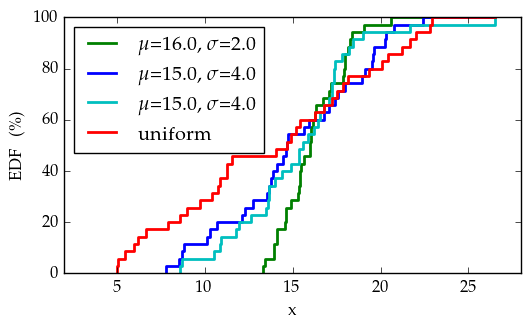
\includegraphics[width=\textwidth]{kuvat/edf.png}
   \caption{Empirical distribution function for four random samples drawn from different normal distributions.}
   \label{fig:edf}
\end{figure}

For astronomers the most well-known of these tests is the Kolmogorov-Smirnov test, which is also known as the KS test. Test statistic is calculated based on empirical distribution functions $\hat{F}_1$ and $\hat{F}_2$ derived from two samples and the test statistic
\begin{equation}
	D = \sup_{x} |\hat{F}_1(x) - \hat{F}_2(x)|
\end{equation}
uses the maximum vertical distance of the e.d.f's as shown in [ehdottomasti kuva tähän]. \citep{feigelson2012modern, bohm2010introduction}




\section{Cluster Analysis}
DBSCAN

\chapter{general simulation thingies}
Data used here from EAGLE which uses modified GADGET-2 which is a tree-code that uses leapfrog, other integrators also briefly introduced?
\section{N-body simulations}
\subsection{Hierarchical Tree Algorithm}
\subsection{Numerical Integrators}
\subsection{Halo Finding with Subfind} %iannuzzi thesis
%merger tree mentioned in todo, is it relevant?

\section{Description of actual simulations used}
Volume, number of particles, compare to other simulations, where better and where maybe worse

Resimulation of interesting regions

Simulation has same parameters as EAGLE
800 Mpc volume used
schaye 2015 paper
DM-only parts: Volker-Springer Gadget and Gadget 2 papers 1999 and 2005 or something,     gravity part is more interesting than SPH 
Zooms can use multiple meshes, only one is used here
gravitational softening

\chapter{Findings from DMO Halo Catalogue Analysis}
\section{Selection of Local Group analogues}
criteria, how many found, what are like (some plots maybe? distributions of masses, separations, velocities or correlations between two of those?). This might be part of previous chapter too (relevant to resimulation)?

\section{Local Anisotropy of the Hubble Flow}
Hopefully there's something at least mildly interesting to report when I get to look at the new data

\subsection{Hubble Flow Fitting}
%
%\begin{figure}
%   \centering
%   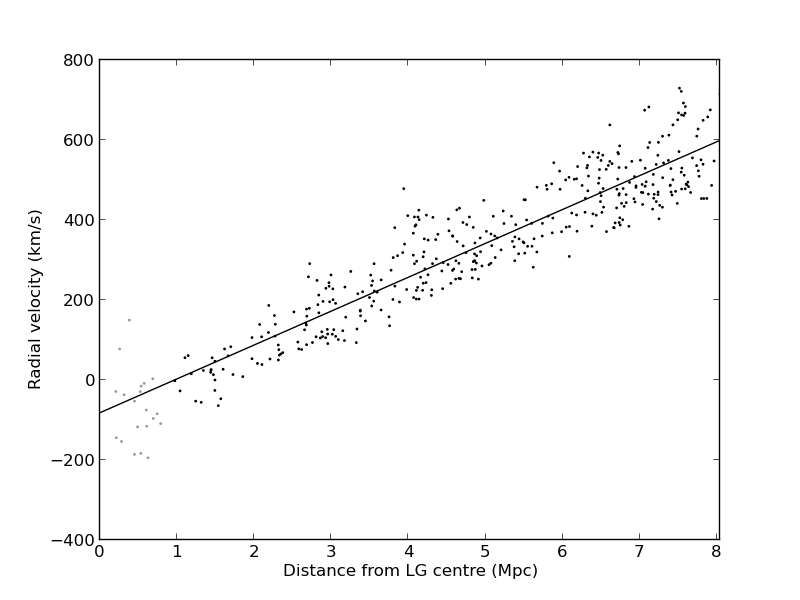
\includegraphics[width=\textwidth]{kuvat/hubbleflow.png}
%   \caption{Radial velocities of haloes as a function of distance. Best fit to Hubble flow shown with solid line. Nearby points ignored when fitting shown in gray.}\label{fig:hubbleflow}
%\end{figure}
%
%\begin{figure}
%   \centering
%   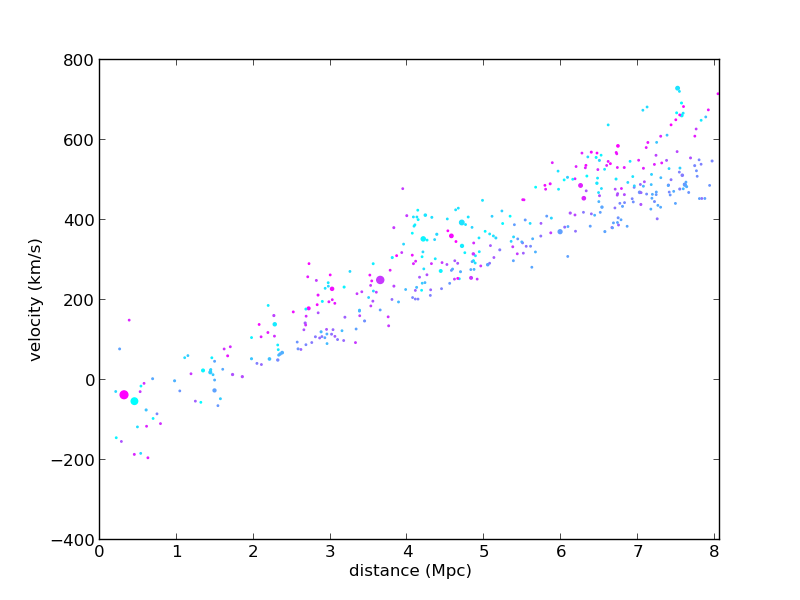
\includegraphics[width=\textwidth]{kuvat/hubbleflow-colour.png}
%   \caption{Hubble flow with colours depicting angular disstance from line connecting Milky Way and Andromeda counterparts in simulation.}\label{fig:hubbleflow-colour}
%\end{figure}
%
%\begin{figure}
%   \centering
%   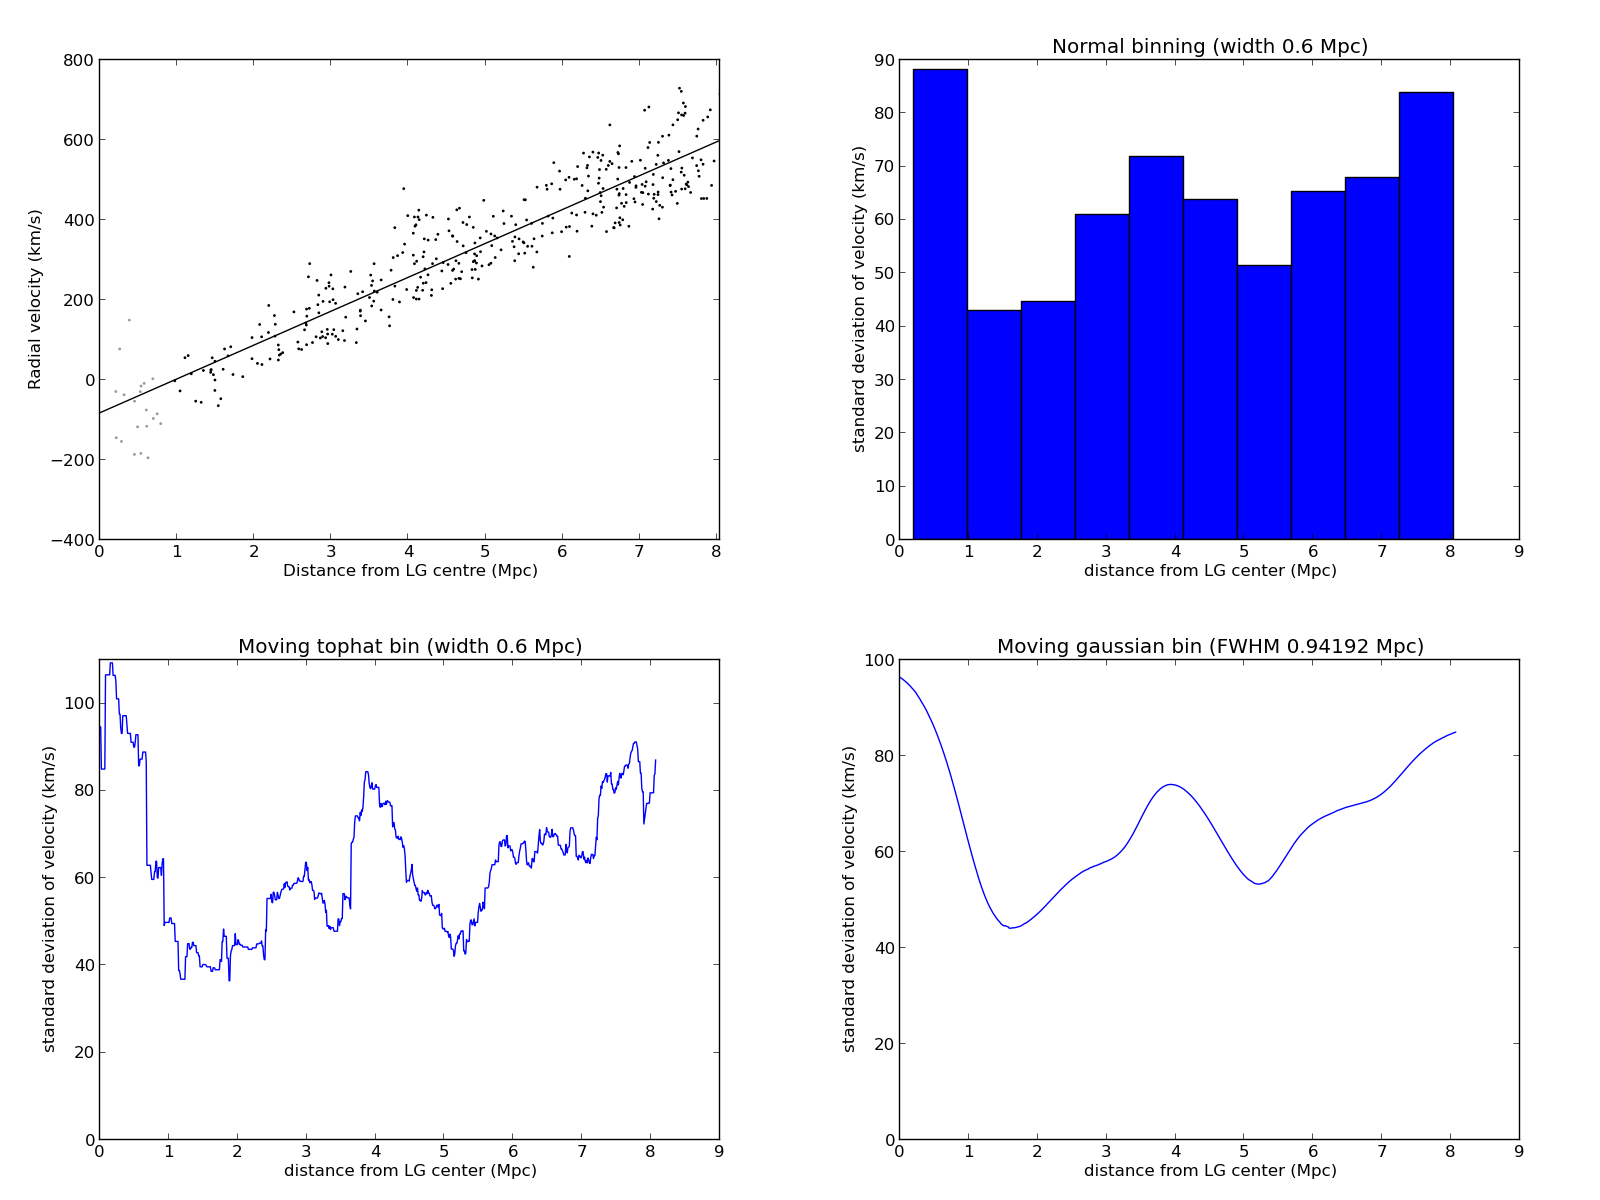
\includegraphics[width=\textwidth]{kuvat/velocitydispersion.png}
%   \caption{Velocity dispersion of Hubble flow.}\label{fig:velocitydispersion}
%\end{figure}
%
%\begin{figure}
%   \centering
%   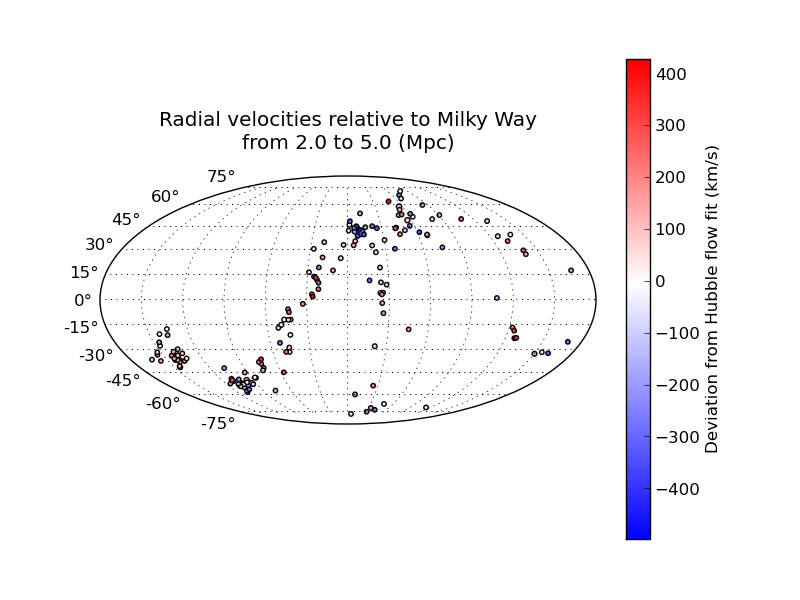
\includegraphics[width=\textwidth]{kuvat/anisotropy-aligned.png}
%   \caption{Haloes with distances between 2 and 5 Mpc as seen from Mily Way counterpart in simulation. Colours depict deviations from best linear Hubble flow fit ignoring haloes up to 2 Mpc away, blue end meaning haloes coming closer faster than expected and redder colours moving away.}\label{fig:anisotropymap}
%\end{figure}
%
%\begin{figure}
%   \centering
%   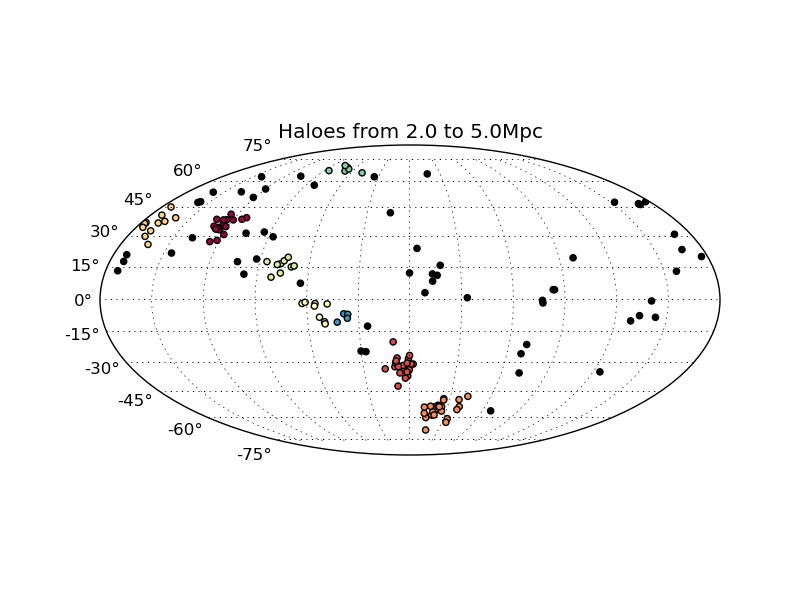
\includegraphics[width=\textwidth]{kuvat/clustering-ms5eps2.png}
%   \caption{Dark matter haloes with distances from 2 to 5 Mpc grouped to clusters using DBSCAN clustering algorithm. Parameters used for this plot were ms=5 and eps=2.}\label{fig:clustering}
%\end{figure}
%
%\begin{figure}
%   \centering
%   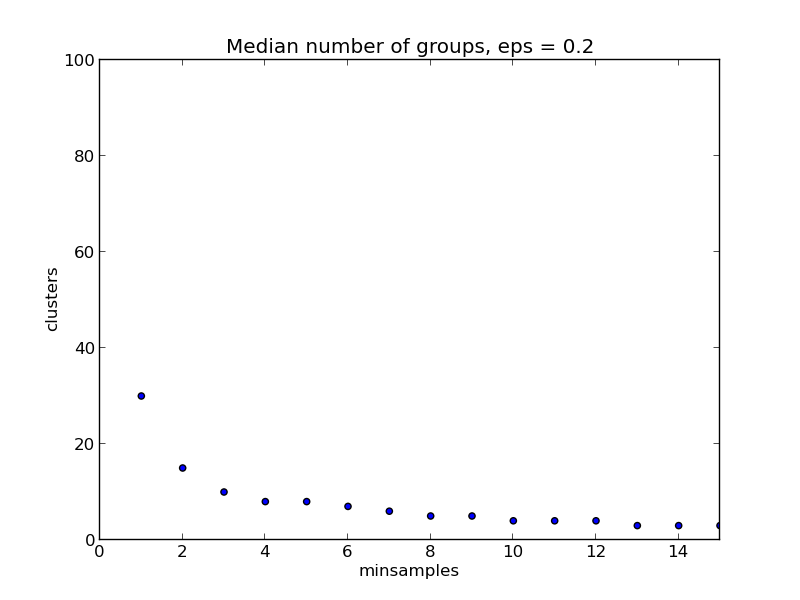
\includegraphics[width=\textwidth]{kuvat/eps-02.png}
%   \caption{Median number of clusters found with constant eps on different minsamples.}\label{fig:epseffect}
%\end{figure}
%
%\begin{figure}
%   \centering
%   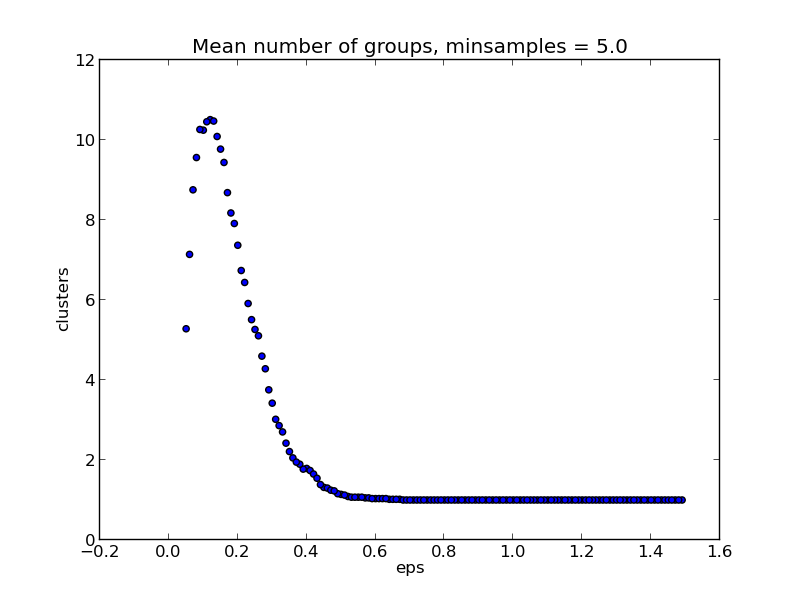
\includegraphics[width=\textwidth]{kuvat/ms-5.png}
%   \caption{Mean number of clusters found with constant ms on different eps.}\label{fig:mseffect}
%\end{figure}
%
%\begin{figure}
%   \centering
%   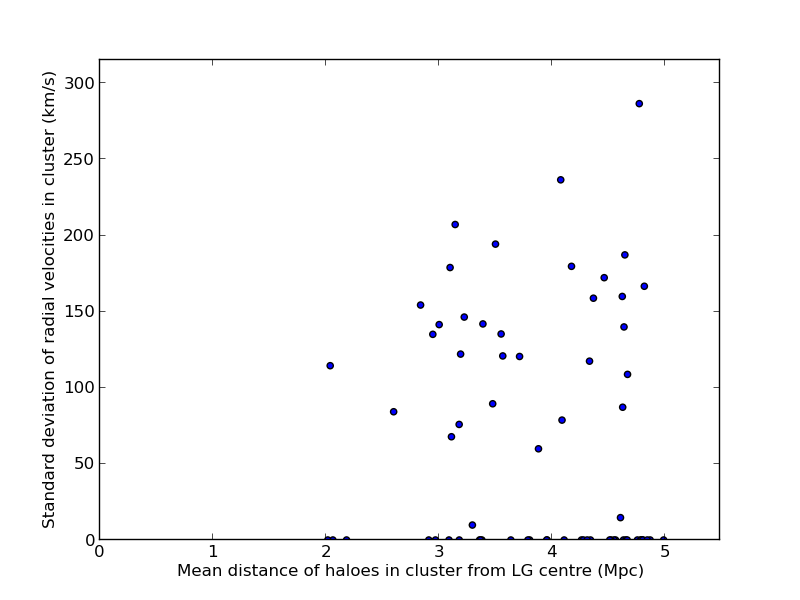
\includegraphics[width=\textwidth]{kuvat/diststd-113.png}
%   \caption{Standard deviation of velocities within cluster as a function of distance.}\label{fig:diststd}
%\end{figure}

\section{Statistical Estimate of the Local Group Mass}
Analysis similar to Fattahi et al 2016 paper

%\chapter{SIBELIUS project}
% Simulations Beyond the Local Universe
%
%\section{Hubble Flow Fitting}
%
% %if results
%\chapter{Conclusions}

\chapter{Conclusions}





% STEP 5:
% Uncomment the following lines and set your .bib file and desired bibliography style
% to make a bibliography with BibTeX.
% Alternatively you can use the thebibliography environment if you want to add all
% references by hand.

\clearpage
\addcontentsline{toc}{chapter}{Bibliography} % This lines adds the bibliography to the ToC
\bibliographystyle{plainnat}
\bibliography{lahteet}


\end{document}

